%
% Presentación de TT uno.
% Proyecto Lovelace.
% Planteamiento de la solución.
%

\section{Planteamiento de la solución}

\subsection{Objetivos del proyecto} % =========================================
\begin{frame}{Objetivos del proyecto}

  Lo que se busca con este proyecto es implementar un programa generador de
  \textit{tokens} que provea confidencialidad a los datos de las tarjetas
  bancarias.

  Además, con el afán de disminuir la desinformación existente sobre la
  tokenización, se busca obtener una comparativa de los algoritmos
  implementados.

\end{frame}

\subsection{Metodología del proyecto} % =======================================
\begin{frame}{Metodología del proyecto}

  \begin{columns}

    \begin{column}{0.5\textwidth}
      Para el desarrollo de este proyecto se está usando una metodología de
      prototipos, en la que cada prototipo usa como metodología interna SDL
      (\textit{Security Development Lifecycle})~\cite{sdl}.
    \end{column}

    \begin{column}{0.5\textwidth}
      \begin{figure}[H]
        \begin{center}
          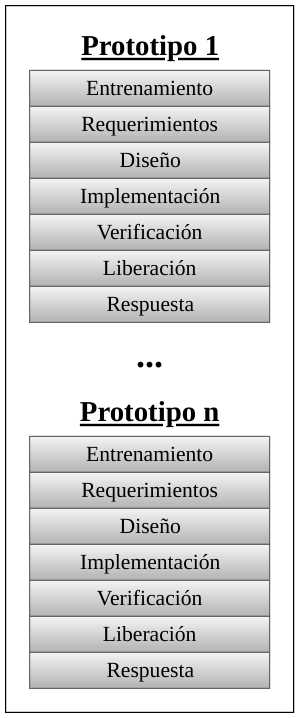
\includegraphics[width=0.5\linewidth]{diagramas/metodologia.png}
          \caption{Fases del trabajo terminal.}
        \end{center}
      \end{figure}
    \end{column}

  \end{columns}

  % SDL es una metodología especializada para software de seguridad desarrollada
  % por Microsoft, que se caracteriza por continuas fases de verificación de
  % seguridad y una primera etapa de estudio de los temas acordes al proyecto.

  % Yo creo que nos podemos saltar la parte de quién la desarrolla.

\end{frame}

\subsection{Prototipos} % =====================================================
\begin{frame}{Prototipos}

  Este proyecto está dividido en 3 prototipos, los cuales son:

  \begin{figure}[H]
    \begin{center}
      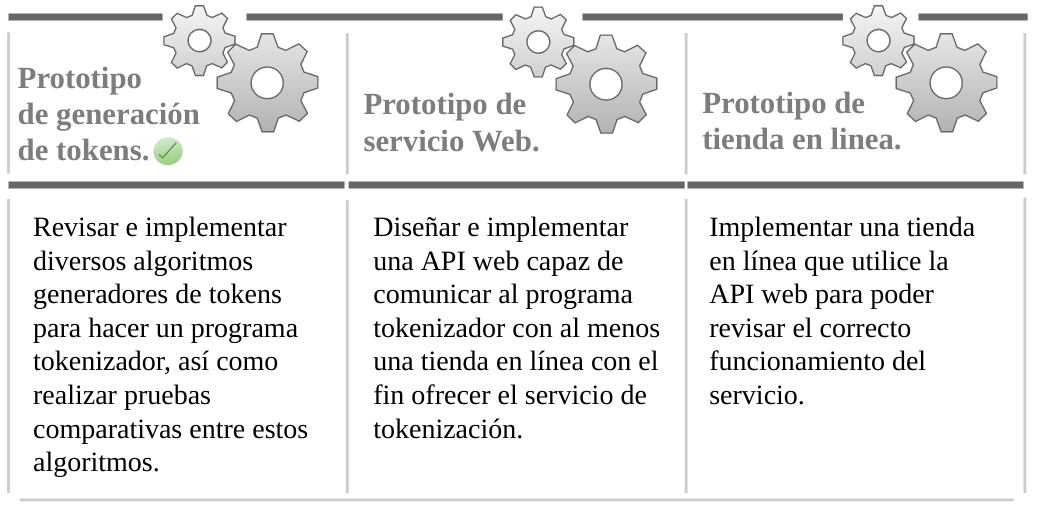
\includegraphics[width=1.0\linewidth]{diagramas/prototipos.png}
      \caption{Prototipos del trabajo terminal.}
    \end{center}
  \end{figure}

\end{frame}

% \subsection{Especificaciones técnicas del desarrollo} % =====================
% \begin{frame}{Especificaciones técnicas del desarrollo}
%
%   % ¿Combina mantenibilidad con «el nivel de rendimiento que ofrece»
%
%   La implementación de los algoritmos generadores de \textit{tokens} se hizo
%   en lenguaje C++, dado que combina mantenibilidad y rendimiento.
%
%   Para las implementaciones que hacen uso de una base de datos, se utilizó
%   el gestor MariaDB, el cual es una bifurcación de MySQL.
%
% \end{frame}
